
\section{Rauch- und Morsezeichen}
\label{section:rauch_und_morsezeichen}
\begin{frame}%STARTCONTENT
\begin{itemize}
  \item Seit Urzeiten versuchen Menschen, Nachrichten über große Entfernungen zu übertragen
  \item Beispielsweise mit Rauchzeichen
  \item Absprache notwendig, welche Bedeutung wie viele Rauchzeichen in einem Zeitabstand haben
  \end{itemize}

\end{frame}

\begin{frame}
\frametitle{Morsezeichen}
\begin{columns}
    \begin{column}{0.48\textwidth}
    \begin{itemize}
  \item Sind ähnlich zu Rauchzeichen
  \item Funkgerät erzeugt mit Oszillator eine Schwingung
  \item Drücken der Morsetaste bringt diese Schwingung auf die Antenne
  \item Empfänger macht diese Aussendung hörbar
  \end{itemize}

    \end{column}
   \begin{column}{0.48\textwidth}
       \begin{itemize}
  \item Unterscheidung zwischen kurzem oder langem Drücken und Pausen möglich
  \end{itemize}

\begin{figure}
    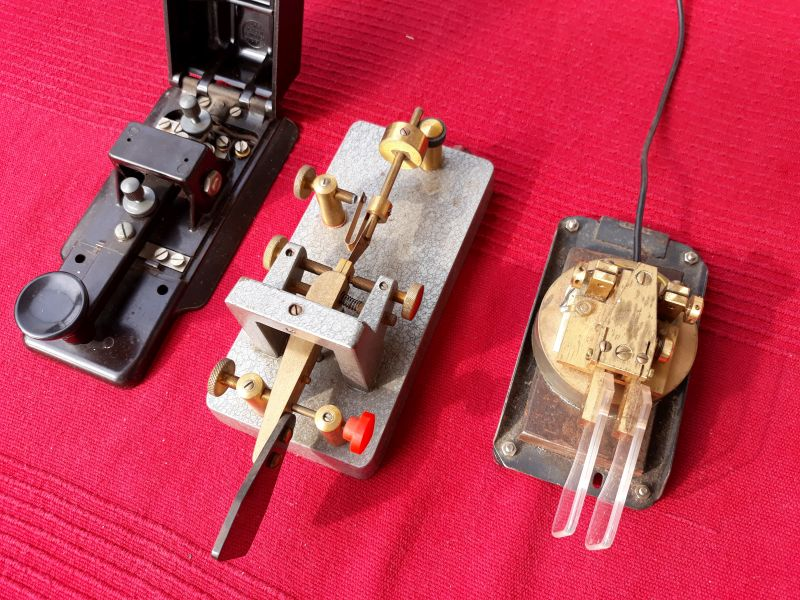
\includegraphics[width=0.85\textwidth]{foto/109}
    \caption{\scriptsize Morsetasten}
    \label{n_cwtast}
\end{figure}

   \end{column}
\end{columns}

\end{frame}

\begin{frame}
\begin{figure}
    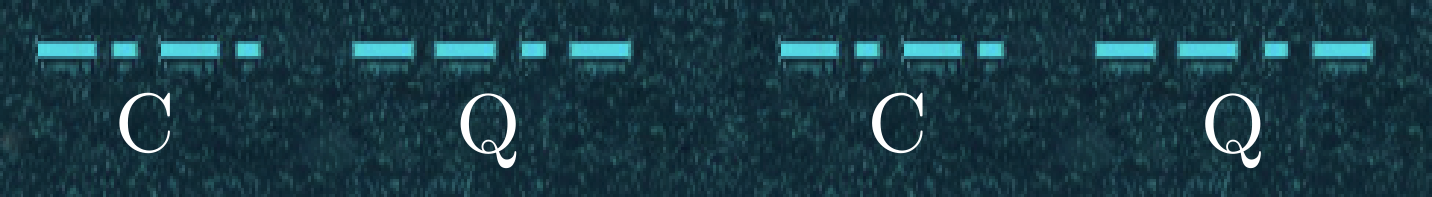
\includegraphics[width=0.85\textwidth]{foto/216}
    \caption{\scriptsize \enquote{CQ CQ} in Morsetelegrafie}
    \label{n_cqcq_horiz}
\end{figure}
\begin{itemize}
  \item Einigung darauf, was bestimmte Abfolgen unterschiedlicher Zeitabstände bedeuten
  \item Mitte des 19. Jahrhunderts Verständigung über den bis heute üblichen Morsecode
  \end{itemize}

\end{frame}

\begin{frame}
\frametitle{Telegrafie}
\begin{itemize}
  \item Übertragungsverfahren mit Hilfsmittel
  \item Rauch oder elektrische Schwingung wird so beeinflusst, um eine Nachricht zu übertragen
  \item Das Hilfsmittel ist der \emph{Träger}
  \item Im Funk aufgrund hoher Frequenzen auch \emph{Hochfrequenz-Träger} oder \emph{HF-Träger}
  \item Verfahren zum Ändern des Trägers ist die \emph{Modulation}
  \end{itemize}

\end{frame}

\begin{frame}
\only<1>{
\begin{QQuestion}{NE201}{Wie werden bei \glqq CW\grqq{} (Continuous Wave) Informationen übertragen?}{Durch Ein- und Ausschalten eines HF-Trägers}
{Durch Änderung der Trägerfrequenz in diskreten Stufen}
{Durch Modulation eines Subträgers}
{Durch diskrete Phasenmodulation}
\end{QQuestion}

}
\only<2>{
\begin{QQuestion}{NE201}{Wie werden bei \glqq CW\grqq{} (Continuous Wave) Informationen übertragen?}{\textbf{\textcolor{DARCgreen}{Durch Ein- und Ausschalten eines HF-Trägers}}}
{Durch Änderung der Trägerfrequenz in diskreten Stufen}
{Durch Modulation eines Subträgers}
{Durch diskrete Phasenmodulation}
\end{QQuestion}

}
\end{frame}

\begin{frame}
\only<1>{
\begin{QQuestion}{NE101}{Durch Modulation~...}{werden dem Signal NF-Komponenten entnommen.}
{wird einem oder mehreren Trägern Informationen entnommen.}
{werden Sprach- und CW-Signale kombiniert.}
{werden Informationen auf einen oder mehrere Träger übertragen.}
\end{QQuestion}

}
\only<2>{
\begin{QQuestion}{NE101}{Durch Modulation~...}{werden dem Signal NF-Komponenten entnommen.}
{wird einem oder mehreren Trägern Informationen entnommen.}
{werden Sprach- und CW-Signale kombiniert.}
{\textbf{\textcolor{DARCgreen}{werden Informationen auf einen oder mehrere Träger übertragen.}}}
\end{QQuestion}

}
\end{frame}

\begin{frame}
\frametitle{Andere Modulationsarten}
Die elektrische Schwingung kann auf andere Arten moduliert werden

\begin{itemize}
  \item Stärke (Amplitude)
  \item Periode (Frequenz)
  \end{itemize}
\end{frame}%ENDCONTENT
